% Für Bindekorrektur als optionales Argument "BCORfaktormitmaßeinheit", dann
% sieht auch Option "twoside" vernünftig aus
% Näheres zu "scrartcl" bzw. "scrreprt" und "scrbook" siehe KOMA-Skript Doku
\documentclass[12pt,a4paper,titlepage,headinclude,bibtotoc]{scrartcl}


%---- Allgemeine Layout Einstellungen ------------------------------------------

% Für Kopf und Fußzeilen, siehe auch KOMA-Skript Doku
\usepackage[komastyle]{scrpage2}
\pagestyle{scrheadings}
\automark[section]{chapter}
\setheadsepline{0.5pt}[\color{black}]

%keine Einrückung
\parindent0pt

%Einstellungen für Figuren- und Tabellenbeschriftungen
\setkomafont{captionlabel}{\sffamily\bfseries}
\setcapindent{0em}

\usepackage{caption}

%---- Weitere Pakete -----------------------------------------------------------
% Die Pakete sind alle in der TeX Live Distribution enthalten. Wichtige Adressen
% www.ctan.org, www.dante.de

% Sprachunterstützung
\usepackage[ngerman]{babel}

% Benutzung von Umlauten direkt im Text
% entweder "latin1" oder "utf8"
\usepackage[utf8]{inputenc}

% Pakete mit Mathesymbolen und zur Beseitigung von Schwächen der Mathe-Umgebung
\usepackage{latexsym,exscale,amssymb,amsmath}
\usepackage{nicefrac}

% Weitere Symbole
\usepackage[nointegrals]{wasysym}
\usepackage{eurosym}

% Anderes Literaturverzeichnisformat
%\usepackage[square,sort&compress]{natbib}

% Für Farbe
\usepackage{color}

% Zur Graphikausgabe
%Beipiel: \includegraphics[width=\textwidth]{grafik.png}
\usepackage{graphicx}

% Text umfließt Graphiken und Tabellen
% Beispiel:
% \begin{wrapfigure}[Zeilenanzahl]{"l" oder "r"}{breite}
%   \centering
%   \includegraphics[width=...]{grafik}
%   \caption{Beschriftung} 
%   \label{fig:grafik}
% \end{wrapfigure}
\usepackage{wrapfig}

% Mehrere Abbildungen nebeneinander
% Beispiel:
% \begin{figure}[htb]
%   \centering
%   \subfigure[Beschriftung 1\label{fig:label1}]
%   {\includegraphics[width=0.49\textwidth]{grafik1}}
%   \hfill
%   \subfigure[Beschriftung 2\label{fig:label2}]
%   {\includegraphics[width=0.49\textwidth]{grafik2}}
%   \caption{Beschriftung allgemein}
%   \label{fig:label-gesamt}
% \end{figure}
\usepackage{subfigure}
\usepackage{adjustbox}

% Caption neben Abbildung
% Beispiel:
% \sidecaptionvpos{figure}{"c" oder "t" oder "b"}
% \begin{SCfigure}[rel. Breite (normalerweise = 1)][hbt]
%   \centering
%   \includegraphics[width=0.5\textwidth]{grafik.png}
%   \caption{Beschreibung}
%   \label{fig:}
% \end{SCfigure}
\usepackage{sidecap}

% Befehl für "Entspricht"-Zeichen
\newcommand{\corresponds}{\ensuremath{\mathrel{\widehat{=}}}}

%Für chemische Formeln (von www.dante.de)
%% Anpassung an LaTeX(2e) von Bernd Raichle
\makeatletter
\DeclareRobustCommand{\chemical}[1]{%
  {\(\m@th
   \edef\resetfontdimens{\noexpand\)%
       \fontdimen16\textfont2=\the\fontdimen16\textfont2
       \fontdimen17\textfont2=\the\fontdimen17\textfont2\relax}%
   \fontdimen16\textfont2=2.7pt \fontdimen17\textfont2=2.7pt
   \mathrm{#1}%
   \resetfontdimens}}
\makeatother

%Si Einheiten
\usepackage{siunitx}

%c++ Code einbinden
\usepackage{listings}
\lstset{numbers=left, numberstyle=\tiny, numbersep=5pt}

%Differential
\newcommand{\dif}{\ensuremath{\mathrm{d}}}

%Boxen,etc.
\usepackage{fancybox}
\usepackage{empheq}

%Fußnoten auf gleiche Seite
\interfootnotelinepenalty=1000

%Dateien aus Unterverzeichnissen
\usepackage{import}

%Bibliography \bibliography{literatur} und \cite{gerthsen}
%\usepackage{cite}
\usepackage{babelbib}
\selectbiblanguage{ngerman}

\begin{document}

\begin{titlepage}
\centering
\textsc{\Large Anfängerpraktikum der Fakultät für
  Physik,\\[1.5ex] Universität Göttingen}

\vspace*{4.2cm}

\rule{\textwidth}{1pt}\\[0.5cm]
{\huge \bfseries
  14\\[1.5ex]
  Wechselstromwiderstände}\\[0.5cm]
\rule{\textwidth}{1pt}

\vspace*{2.5cm}

\begin{Large}
\begin{tabular}{ll}
Praktikant: & Felix Kurtz\\
Versuchspartner: & Michael Lohmann\\
 E-Mail: &  felix.kurtz@stud.uni-goettingen.de\\
 Betreuer: & Björn Klaas\\
 Versuchsdatum: & 08.09.2014\\
\end{tabular}
\end{Large}

\vspace*{0.8cm}

\begin{Large}
\fbox{
  \begin{minipage}[t][2.5cm][t]{6cm} 
   Eingegangen am:
  \end{minipage}
}
\end{Large}

\end{titlepage}

\tableofcontents

\newpage

\section{Einleitung}
\label{sec:einleitung}
Bei diesem Versuch sollen neben ohmschen Widerständen induktive und kapazitive Widerstände und die damit verbundene Phasenverschiebung zwischen Strom und Spannung bei Wechselstrom untersucht werden.
Gegenstand der Messungen ist die Reihenschaltung aus Widerstand, Spule und Kondensator und die dabei auftretende Resonanz.
Außerdem wird die Parallelschaltung aus Spule und Kondensator betrachtet.

\section{Theorie}
\label{sec:theorie}
\subsection{Wechselstrom}
Bei dem heutzutage fast überall verwendeten \textit{Wechselstrom} verhalten sich Spannung und Strom Sinus-förmig, sind jedoch um $\varphi$ phasenverschoben:
\begin{align}
	U(t)&=U_0\cdot\sin(\omega t)\,,\\
	I(t)&=I_0\cdot\sin(\omega t-\varphi)\,.
\end{align}

\subsubsection{Effektivwerte}
Als \textit{Effektivwert} eines Wechselstroms bezeichnet man den Wert, bei dem bei Gleichstrom die gleiche Leistung abgegeben würde.
Für eine Sinus-förmige Spannung der Amplitude $U_0$ ergibt sich somit
\begin{align}
	U_\text{eff}=\sqrt{\frac{1}{2}}\cdot U_0 \,.
\end{align}
Analoges gilt für den Strom.
Vom Multimeter, welches Wechselstrom misst, wird der Effektivwert und nicht die Amplitude der Messgröße angezeigt.

\subsubsection{Impedanz und Scheinwiderstand}
Für die folgende Rechnung ist es nützlich, die komplexe Schreibweise $U(t)=U_0 \, e^{i\omega t}$ und $I(t)=I_0 \, e^{i(\omega t - \varphi)}$ zu verwenden.
Als Impedanz bezeichnet man das Verhältnis
\begin{align}
	Z=\frac{U(t)}{I(t)}=\frac{U_0}{I_0}\cdot e^{i\varphi}\,.
\end{align}
Ihr Betrag ist der Scheinwiderstand $|Z|=\frac{U_0}{I_0}=\frac{U_\text{eff}}{I_\text{eff}}$.

\subsection{Ohmscher Widerstand}
Bei einem ohmschen Widerstand $R$ gilt immer
\begin{align}
	U(t)=R \cdot I(t)\,.
\end{align}
Strom und Spannung sind also in Phase.

\subsection{Kapazitiver Widerstand}
Ein Kondensator mit der Kapazität $C$, an dem die Spannung $U$ anliegt, trägt die Ladung $Q=C\cdot U$.
Für eine Wechselspannung $U_0\sin(\omega t)$ ergibt sich aus der zeitlichen Ableitung der Ladung $I=\dot{Q}$
\begin{align}
	I(t)=\omega C\cdot U_0\cdot \cos(\omega t)=\omega C\cdot U_0\cdot\sin\left(\omega t+\frac{\pi}{2}\right)\,.
\end{align}
Man erkennt, dass der Strom der Spannung voraus eilt und die Phasenverschiebung $\varphi=-\frac{\pi}{2}$ beträgt.
Über die komplexe Schreibweise lässt sich der rein imaginäre \textit{Blindwiderstand}
\begin{align}
	X_C=\frac{U}{I}= \frac{U_0}{\omega C \cdot U_0}\, e^{-i\frac{\pi}{2}}=-i\frac{1}{\omega C}
\end{align}
definieren.

\subsection{Induktiver Widerstand}
Fließt durch eine Spule mit der Induktivität $L$ ein zeitlich veränderlicher Strom, induziert dieser eine Induktionsspannung $U_\text{ind}=-L\dot{I}$.
Soll diese Spannung die Form $U_0\,\sin(\omega t)$, folgt für den Strom durch Integration
\begin{align}
	I(t)=\frac{U_0}{\omega L}\cdot \sin\left(\omega t-\frac{\pi}{2}\right)\,.
\end{align}
Für den Blindwiderstand gilt also
\begin{align}
	X_L=i\omega L \,.
\end{align}
Hier eilt die Spannung also dem Strom voraus und die Phasenverschiebung beträgt $\varphi=\frac{\pi}{2}$.
Außerdem ist $X_L$ größer, je größer die Frequenz $\omega$ des Wechselstroms.

Außerdem besitzen Spulen meist einen nicht zu vernachlässigenden ohmschen Widerstand $R_L$, da sie aus sehr langem Draht bestehen.

\subsection{RLC-Serienschaltung}
Schaltet man einen ohmschen Widerstand $R$, eine Spule mit der Induktivität $L$ und einen Kondensator mit der Kapazität $C$ in Reihe ist die Impedanz die Summe aus ohmschem, kapazitivem sowie induktivem Widerstand
\begin{align}
	Z=R+X_C+X_L \,.
\end{align}
Der Scheinwiderstand beträgt folglich
\begin{align}
	|Z|=\sqrt{R^2+\left(\omega L - \frac{1}{\omega C}\right)^2} \,.
	\label{eq:Scheinwiderstand_serie}
\end{align}
Außerdem kann man alle drei Widerstände in die komplexe Ebene einzeichnen.
Dabei ist der ohmsche Widerstand auf der reelen Achse und die beiden Blindwiderstände auf der imaginären Achse.
Addiert man alle, ergibt sich die Impedanz.
Der Winkel zwischen $Z$ und der reelen Achse ist die Phasenverschiebung $\phi$ zwischen Spannung und Strom 
Sie kann also mit der Formel 
\begin{align}
	\varphi=\arctan\left(\frac{\omega L - \frac{1}{\omega C}}{R} \right)
	\label{eq:phase_serie}
\end{align}
berechnet werden.

Bei der \textbf{Resonanzfrequenz} $\omega_R$ ist der Scheinwiderstand am geringsten, die Blindwiderstände heben sich nämlich auf: $\omega_R L=\frac{1}{\omega_R C}$.
Daraus folgt:
\begin{align}
	\omega_R&=\sqrt{\frac{1}{LC}}
	\label{eq:omega_R}	
	\,,\\
	\varphi(\omega_R)&=0\,,\\
	Z(\omega_R)&=R\,.
\end{align}

\subsection{Parallelschaltung}
Schaltet man eine Spule mit der Induktivität $L$ und dem ohmschen Widerstand $R_L$ parallel zu einem Kondensator mit der Kapazität $C$, ergibt sich für die Impedanz
\begin{align}
	Z(\omega)=\left(\frac{1}{R_L+i\omega L}+i\omega C\right)^{-1}\
\end{align}
und
\begin{align}
	|Z|=\left[\left(\omega C - \frac{\omega L}{R_L^2+(\omega L)^2}\right)^2+	\left(\frac{R_L}{R_L^2+(\omega L)^2}\right)^2\right]^{-\frac{1}{2}}
	\label{eq:parallel}
\end{align}
als Scheinwiderstand.
                                                                                                                                                                      
\section{Durchführung}
\label{sec:durchfuehrung}
\begin{figure}[!htb]
	\centering
	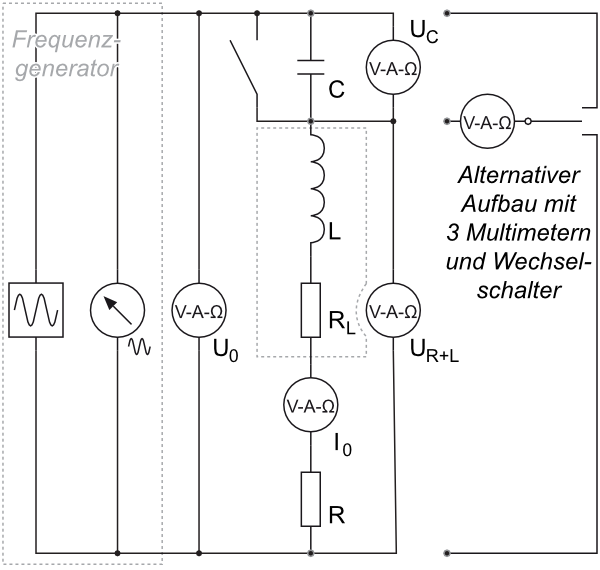
\includegraphics[scale=0.6]{serie.png}
	\caption{RLC-Serienschaltung \cite[Datum: 03.10.14]{LP14}.}
	\label{fig:serie}
\end{figure}

Zuerst wird der \textbf{Serienresonanzkreis} aus Abb. \ref{fig:serie} aufgebaut.
Dabei wird das Oszilloskop so angeschlossen und eingestellt, dass die Phasenverschiebung zwischen Strom und Spannung abgelesen werden kann:
Während die Spannung parallel zum Frequenzgenerator gemessen wird und an Channel 1 des Oszilloskops anliegt, legt man in die Stromzange (Channel 2) das Kabel, von welchem der Strom gemessen werden soll.
Nun schaltet man im y-t-Mode des Oszilloskops unter dem Punkt \emph{Messung} die Bestimmung der Phasenverschiebung zwischen den beiden Signalen ein.\\
Zur ersten Messung überbrückt man den Kondensator, indem man den Schalter schließt.
Nun wird für mindestens 10 Frequenzen Spannung und Strom sowie deren Phasenverschiebung gemessen.
Daraus kann man später die Induktivität der Spule sowie den ohmschen Widerstand berechnen.\\
Die nächsten Messungen finden mit dem Kondensator statt, der Schalter wird also geöffnet.
In Abhängigkeit der Frequenz werden jetzt der Strom $I$, die Spannung $U$ sowie die Teilspannungen $U_C$ und $U_{L+R}$ und die Phasenverschiebung $\varphi$ gemessen.
Dabei sollen möglichst viele Messungen in der Nähe der Resonanzfrequenz $\omega_R$ durchgeführt werden.\\

\begin{figure}[!htb]
	\centering
	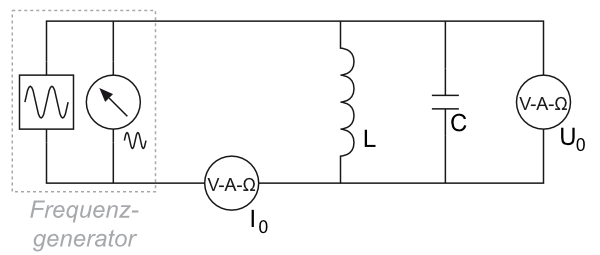
\includegraphics[scale=0.7]{parallel.png}
	\caption{LC-Parallelschaltung \cite[Datum: 03.10.14]{LP14}.}
	\label{fig:parallel}
\end{figure}


Als nächstes wird die Schaltung nach Abb. \ref{fig:parallel} zu einem \textbf{Parallelkreis} aus Spule und Kondensator umgebaut.
Wieder wird die Spannung und der Strom in Abhängigkeit der Frequenz gemessen.
Auch hier liegt der Fokus auf der Resonanzfrequenz.\\

Zum Schluss misst man mit dem Multimeter den Innenwiderstand des Amperemeters und den einzelnen ohmschen Widerstand $R_\Omega$ sowie $R_L$ der Spule.
Außerdem werden die Kapazität des Kondensators gemessen und die Spulendaten notiert. 

\section{Auswertung}
\label{sec:auswertung}
\subsection{Widerstand und Spule in Reihe}
\begin{figure}[!htb]
	\centering
	% GNUPLOT: LaTeX picture with Postscript
\begingroup
  \makeatletter
  \providecommand\color[2][]{%
    \GenericError{(gnuplot) \space\space\space\@spaces}{%
      Package color not loaded in conjunction with
      terminal option `colourtext'%
    }{See the gnuplot documentation for explanation.%
    }{Either use 'blacktext' in gnuplot or load the package
      color.sty in LaTeX.}%
    \renewcommand\color[2][]{}%
  }%
  \providecommand\includegraphics[2][]{%
    \GenericError{(gnuplot) \space\space\space\@spaces}{%
      Package graphicx or graphics not loaded%
    }{See the gnuplot documentation for explanation.%
    }{The gnuplot epslatex terminal needs graphicx.sty or graphics.sty.}%
    \renewcommand\includegraphics[2][]{}%
  }%
  \providecommand\rotatebox[2]{#2}%
  \@ifundefined{ifGPcolor}{%
    \newif\ifGPcolor
    \GPcolortrue
  }{}%
  \@ifundefined{ifGPblacktext}{%
    \newif\ifGPblacktext
    \GPblacktexttrue
  }{}%
  % define a \g@addto@macro without @ in the name:
  \let\gplgaddtomacro\g@addto@macro
  % define empty templates for all commands taking text:
  \gdef\gplbacktext{}%
  \gdef\gplfronttext{}%
  \makeatother
  \ifGPblacktext
    % no textcolor at all
    \def\colorrgb#1{}%
    \def\colorgray#1{}%
  \else
    % gray or color?
    \ifGPcolor
      \def\colorrgb#1{\color[rgb]{#1}}%
      \def\colorgray#1{\color[gray]{#1}}%
      \expandafter\def\csname LTw\endcsname{\color{white}}%
      \expandafter\def\csname LTb\endcsname{\color{black}}%
      \expandafter\def\csname LTa\endcsname{\color{black}}%
      \expandafter\def\csname LT0\endcsname{\color[rgb]{1,0,0}}%
      \expandafter\def\csname LT1\endcsname{\color[rgb]{0,1,0}}%
      \expandafter\def\csname LT2\endcsname{\color[rgb]{0,0,1}}%
      \expandafter\def\csname LT3\endcsname{\color[rgb]{1,0,1}}%
      \expandafter\def\csname LT4\endcsname{\color[rgb]{0,1,1}}%
      \expandafter\def\csname LT5\endcsname{\color[rgb]{1,1,0}}%
      \expandafter\def\csname LT6\endcsname{\color[rgb]{0,0,0}}%
      \expandafter\def\csname LT7\endcsname{\color[rgb]{1,0.3,0}}%
      \expandafter\def\csname LT8\endcsname{\color[rgb]{0.5,0.5,0.5}}%
    \else
      % gray
      \def\colorrgb#1{\color{black}}%
      \def\colorgray#1{\color[gray]{#1}}%
      \expandafter\def\csname LTw\endcsname{\color{white}}%
      \expandafter\def\csname LTb\endcsname{\color{black}}%
      \expandafter\def\csname LTa\endcsname{\color{black}}%
      \expandafter\def\csname LT0\endcsname{\color{black}}%
      \expandafter\def\csname LT1\endcsname{\color{black}}%
      \expandafter\def\csname LT2\endcsname{\color{black}}%
      \expandafter\def\csname LT3\endcsname{\color{black}}%
      \expandafter\def\csname LT4\endcsname{\color{black}}%
      \expandafter\def\csname LT5\endcsname{\color{black}}%
      \expandafter\def\csname LT6\endcsname{\color{black}}%
      \expandafter\def\csname LT7\endcsname{\color{black}}%
      \expandafter\def\csname LT8\endcsname{\color{black}}%
    \fi
  \fi
  \setlength{\unitlength}{0.0500bp}%
  \begin{picture}(7200.00,5040.00)%
    \gplgaddtomacro\gplbacktext{%
      \csname LTb\endcsname%
      \put(946,704){\makebox(0,0)[r]{\strut{} 0}}%
      \put(946,1213){\makebox(0,0)[r]{\strut{} 0.2}}%
      \put(946,1722){\makebox(0,0)[r]{\strut{} 0.4}}%
      \put(946,2231){\makebox(0,0)[r]{\strut{} 0.6}}%
      \put(946,2740){\makebox(0,0)[r]{\strut{} 0.8}}%
      \put(946,3248){\makebox(0,0)[r]{\strut{} 1}}%
      \put(946,3757){\makebox(0,0)[r]{\strut{} 1.2}}%
      \put(946,4266){\makebox(0,0)[r]{\strut{} 1.4}}%
      \put(946,4775){\makebox(0,0)[r]{\strut{} 1.6}}%
      \put(1078,484){\makebox(0,0){\strut{} 0}}%
      \put(1651,484){\makebox(0,0){\strut{} 1}}%
      \put(2223,484){\makebox(0,0){\strut{} 2}}%
      \put(2796,484){\makebox(0,0){\strut{} 3}}%
      \put(3368,484){\makebox(0,0){\strut{} 4}}%
      \put(3941,484){\makebox(0,0){\strut{} 5}}%
      \put(4513,484){\makebox(0,0){\strut{} 6}}%
      \put(5086,484){\makebox(0,0){\strut{} 7}}%
      \put(5658,484){\makebox(0,0){\strut{} 8}}%
      \put(6231,484){\makebox(0,0){\strut{} 9}}%
      \put(6803,484){\makebox(0,0){\strut{} 10}}%
      \put(176,2739){\rotatebox{-270}{\makebox(0,0){\strut{}$|Z|^2$ [(k$\Omega )^2$]}}}%
      \put(3940,154){\makebox(0,0){\strut{}$\omega^2$ [(kHz)$^2$]}}%
    }%
    \gplgaddtomacro\gplfronttext{%
      \csname LTb\endcsname%
      \put(3454,4602){\makebox(0,0)[r]{\strut{}Messwerte}}%
      \csname LTb\endcsname%
      \put(3454,4382){\makebox(0,0)[r]{\strut{}Regressionsgerade}}%
    }%
    \gplbacktext
    \put(0,0){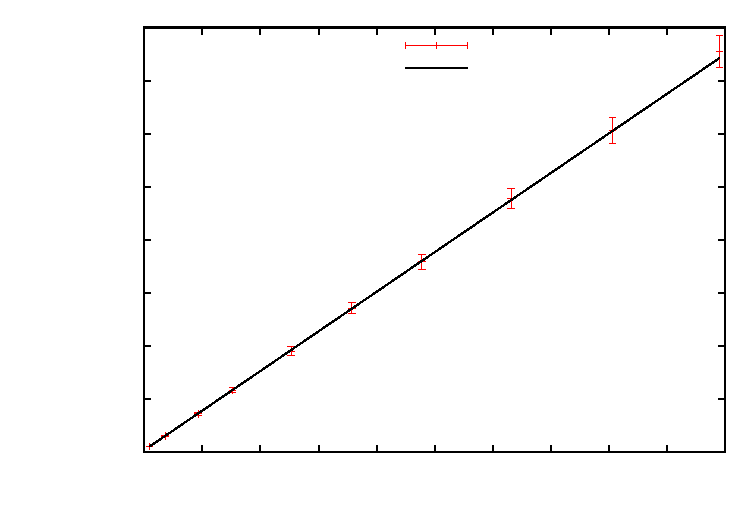
\includegraphics{messung1}}%
    \gplfronttext
  \end{picture}%
\endgroup

	\caption{RL-Serienschaltung: Quadrat des Scheinwiderstandes als Funktion der Kreisfrequenz.}
	\label{fig:messung1}
\end{figure}
Trägt man das Quadrat der Impedanz gegen das der Kreisfrequenz auf, ergibt sich eine Gerade $Z^2=R^2+L^2\omega^2=b+m\cdot(\omega^2)$.
Dies kann man in Abb. \ref{fig:messung1} erkennen.
Um aus dem Ergebnis der linearen Regression $m$ und $b$ die Induktivität  $L$ sowie den ohmschen Widerstand $R$ zu berechnen, muss also die Wurzel gezogen werden.
Der Fehler von $x=\sqrt{y}$ berechnet man mit der Formel $\sigma_x=\frac{\sigma_y}{2\sqrt{y}}$, welche aus der Gauss'schen  Fehlerfortpflanzung stammt.

So erhält man aus $m = (0.1493 \pm 0.0005)\,\si{\ohm^2\per\hertz^2}$ und $b = (0.00597 \pm 0.00017)\,\si{(\kilo\ohm)^2}$ 
\begin{align*}
	L&=(386.3\pm 0.6)\,\si{\milli\henry}\qquad \text{sowie}\\
	R&=(77.3 \pm 1.1)\,\si{\ohm}\,.
\end{align*}
\subsection{RLC-Serienschaltung}
\subsubsection{Scheinwiderstand}
\begin{figure}[!htb]
	\centering
	% GNUPLOT: LaTeX picture with Postscript
\begingroup
  \makeatletter
  \providecommand\color[2][]{%
    \GenericError{(gnuplot) \space\space\space\@spaces}{%
      Package color not loaded in conjunction with
      terminal option `colourtext'%
    }{See the gnuplot documentation for explanation.%
    }{Either use 'blacktext' in gnuplot or load the package
      color.sty in LaTeX.}%
    \renewcommand\color[2][]{}%
  }%
  \providecommand\includegraphics[2][]{%
    \GenericError{(gnuplot) \space\space\space\@spaces}{%
      Package graphicx or graphics not loaded%
    }{See the gnuplot documentation for explanation.%
    }{The gnuplot epslatex terminal needs graphicx.sty or graphics.sty.}%
    \renewcommand\includegraphics[2][]{}%
  }%
  \providecommand\rotatebox[2]{#2}%
  \@ifundefined{ifGPcolor}{%
    \newif\ifGPcolor
    \GPcolortrue
  }{}%
  \@ifundefined{ifGPblacktext}{%
    \newif\ifGPblacktext
    \GPblacktexttrue
  }{}%
  % define a \g@addto@macro without @ in the name:
  \let\gplgaddtomacro\g@addto@macro
  % define empty templates for all commands taking text:
  \gdef\gplbacktext{}%
  \gdef\gplfronttext{}%
  \makeatother
  \ifGPblacktext
    % no textcolor at all
    \def\colorrgb#1{}%
    \def\colorgray#1{}%
  \else
    % gray or color?
    \ifGPcolor
      \def\colorrgb#1{\color[rgb]{#1}}%
      \def\colorgray#1{\color[gray]{#1}}%
      \expandafter\def\csname LTw\endcsname{\color{white}}%
      \expandafter\def\csname LTb\endcsname{\color{black}}%
      \expandafter\def\csname LTa\endcsname{\color{black}}%
      \expandafter\def\csname LT0\endcsname{\color[rgb]{1,0,0}}%
      \expandafter\def\csname LT1\endcsname{\color[rgb]{0,1,0}}%
      \expandafter\def\csname LT2\endcsname{\color[rgb]{0,0,1}}%
      \expandafter\def\csname LT3\endcsname{\color[rgb]{1,0,1}}%
      \expandafter\def\csname LT4\endcsname{\color[rgb]{0,1,1}}%
      \expandafter\def\csname LT5\endcsname{\color[rgb]{1,1,0}}%
      \expandafter\def\csname LT6\endcsname{\color[rgb]{0,0,0}}%
      \expandafter\def\csname LT7\endcsname{\color[rgb]{1,0.3,0}}%
      \expandafter\def\csname LT8\endcsname{\color[rgb]{0.5,0.5,0.5}}%
    \else
      % gray
      \def\colorrgb#1{\color{black}}%
      \def\colorgray#1{\color[gray]{#1}}%
      \expandafter\def\csname LTw\endcsname{\color{white}}%
      \expandafter\def\csname LTb\endcsname{\color{black}}%
      \expandafter\def\csname LTa\endcsname{\color{black}}%
      \expandafter\def\csname LT0\endcsname{\color{black}}%
      \expandafter\def\csname LT1\endcsname{\color{black}}%
      \expandafter\def\csname LT2\endcsname{\color{black}}%
      \expandafter\def\csname LT3\endcsname{\color{black}}%
      \expandafter\def\csname LT4\endcsname{\color{black}}%
      \expandafter\def\csname LT5\endcsname{\color{black}}%
      \expandafter\def\csname LT6\endcsname{\color{black}}%
      \expandafter\def\csname LT7\endcsname{\color{black}}%
      \expandafter\def\csname LT8\endcsname{\color{black}}%
    \fi
  \fi
  \setlength{\unitlength}{0.0500bp}%
  \begin{picture}(7200.00,5040.00)%
    \gplgaddtomacro\gplbacktext{%
      \csname LTb\endcsname%
      \put(946,704){\makebox(0,0)[r]{\strut{} 0}}%
      \put(946,1156){\makebox(0,0)[r]{\strut{} 0.2}}%
      \put(946,1609){\makebox(0,0)[r]{\strut{} 0.4}}%
      \put(946,2061){\makebox(0,0)[r]{\strut{} 0.6}}%
      \put(946,2513){\makebox(0,0)[r]{\strut{} 0.8}}%
      \put(946,2966){\makebox(0,0)[r]{\strut{} 1}}%
      \put(946,3418){\makebox(0,0)[r]{\strut{} 1.2}}%
      \put(946,3870){\makebox(0,0)[r]{\strut{} 1.4}}%
      \put(946,4323){\makebox(0,0)[r]{\strut{} 1.6}}%
      \put(946,4775){\makebox(0,0)[r]{\strut{} 1.8}}%
      \put(1078,484){\makebox(0,0){\strut{} 0}}%
      \put(1794,484){\makebox(0,0){\strut{} 0.5}}%
      \put(2509,484){\makebox(0,0){\strut{} 1}}%
      \put(3225,484){\makebox(0,0){\strut{} 1.5}}%
      \put(3941,484){\makebox(0,0){\strut{} 2}}%
      \put(4656,484){\makebox(0,0){\strut{} 2.5}}%
      \put(5372,484){\makebox(0,0){\strut{} 3}}%
      \put(6087,484){\makebox(0,0){\strut{} 3.5}}%
      \put(6803,484){\makebox(0,0){\strut{} 4}}%
      \put(176,2739){\rotatebox{-270}{\makebox(0,0){\strut{}Impedanz [k$\Omega$]}}}%
      \put(3940,154){\makebox(0,0){\strut{}Kreisfrequenz [kHz]}}%
    }%
    \gplgaddtomacro\gplfronttext{%
      \csname LTb\endcsname%
      \put(5816,4602){\makebox(0,0)[r]{\strut{}Messwerte}}%
      \csname LTb\endcsname%
      \put(5816,4382){\makebox(0,0)[r]{\strut{}Fit}}%
    }%
    \gplbacktext
    \put(0,0){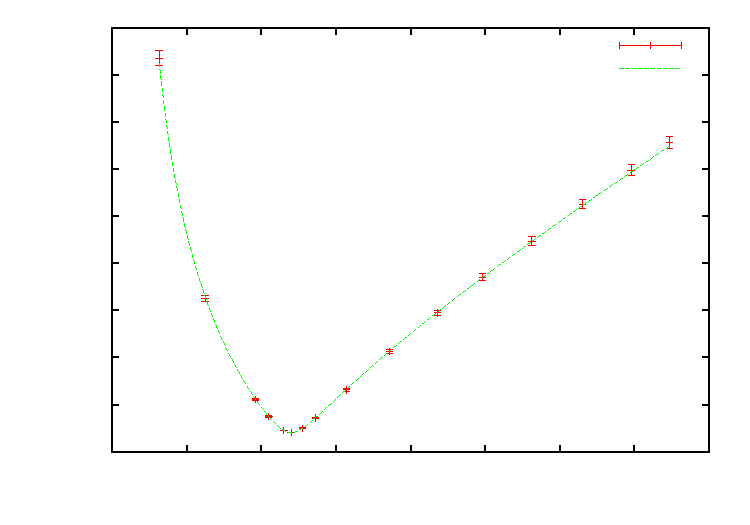
\includegraphics{messung2}}%
    \gplfronttext
  \end{picture}%
\endgroup

	\caption{Scheinwiderstand des Serienresonanzkreises als Funktion der Kreisfrequenz.}
	\label{fig:messung2}
\end{figure}
Trägt man den Scheinwiderstand der Serienschaltung in Abhängigkeit der Frequenz auf (Abb.\ref{fig:messung2}) und fittet die theoretische Kurve aus Formel \eqref{eq:Scheinwiderstand_serie}, erhält man für die Parameter 
\begin{align*}
	R &= (80.9 \pm 0.5)\,\si{\ohm}\,,\\
	L &= (386.1 \pm 1.0)\,\si{\milli\henry}\qquad\text{und}\\
	C &= (1.799 \pm 0.005)\,\si{\micro\farad}\,.
\end{align*}
Mit der Formel \eqref{eq:omega_R} kann nun die Resonanzfrequenz bestimmt werden.
Dabei wird die Formel
\begin{align}
	\sigma_{\omega_R}&=\frac{\sqrt{\frac{\sigma_{L}^{2}}{L^{2}} + \frac{\sigma_{C}^{2}}{C^{2}}}}{2 \cdot \sqrt{C} \cdot \sqrt{L}}\,,
	\label{eq:omega_R_fehler}
\end{align}
die sich aus der Fehlerfortpflanzung ergibt, für den Fehler verwendet.
Man erhält:
\begin{empheq}[box=\shadowbox*]{align*}
	\omega_R&=(1199.9 \pm 2.3)\,\si\hertz \,.
\end{empheq}
\subsubsection{Phasenverschiebung}
\begin{figure}[!htb]
	\centering
	% GNUPLOT: LaTeX picture with Postscript
\begingroup
  \makeatletter
  \providecommand\color[2][]{%
    \GenericError{(gnuplot) \space\space\space\@spaces}{%
      Package color not loaded in conjunction with
      terminal option `colourtext'%
    }{See the gnuplot documentation for explanation.%
    }{Either use 'blacktext' in gnuplot or load the package
      color.sty in LaTeX.}%
    \renewcommand\color[2][]{}%
  }%
  \providecommand\includegraphics[2][]{%
    \GenericError{(gnuplot) \space\space\space\@spaces}{%
      Package graphicx or graphics not loaded%
    }{See the gnuplot documentation for explanation.%
    }{The gnuplot epslatex terminal needs graphicx.sty or graphics.sty.}%
    \renewcommand\includegraphics[2][]{}%
  }%
  \providecommand\rotatebox[2]{#2}%
  \@ifundefined{ifGPcolor}{%
    \newif\ifGPcolor
    \GPcolortrue
  }{}%
  \@ifundefined{ifGPblacktext}{%
    \newif\ifGPblacktext
    \GPblacktexttrue
  }{}%
  % define a \g@addto@macro without @ in the name:
  \let\gplgaddtomacro\g@addto@macro
  % define empty templates for all commands taking text:
  \gdef\gplbacktext{}%
  \gdef\gplfronttext{}%
  \makeatother
  \ifGPblacktext
    % no textcolor at all
    \def\colorrgb#1{}%
    \def\colorgray#1{}%
  \else
    % gray or color?
    \ifGPcolor
      \def\colorrgb#1{\color[rgb]{#1}}%
      \def\colorgray#1{\color[gray]{#1}}%
      \expandafter\def\csname LTw\endcsname{\color{white}}%
      \expandafter\def\csname LTb\endcsname{\color{black}}%
      \expandafter\def\csname LTa\endcsname{\color{black}}%
      \expandafter\def\csname LT0\endcsname{\color[rgb]{1,0,0}}%
      \expandafter\def\csname LT1\endcsname{\color[rgb]{0,1,0}}%
      \expandafter\def\csname LT2\endcsname{\color[rgb]{0,0,1}}%
      \expandafter\def\csname LT3\endcsname{\color[rgb]{1,0,1}}%
      \expandafter\def\csname LT4\endcsname{\color[rgb]{0,1,1}}%
      \expandafter\def\csname LT5\endcsname{\color[rgb]{1,1,0}}%
      \expandafter\def\csname LT6\endcsname{\color[rgb]{0,0,0}}%
      \expandafter\def\csname LT7\endcsname{\color[rgb]{1,0.3,0}}%
      \expandafter\def\csname LT8\endcsname{\color[rgb]{0.5,0.5,0.5}}%
    \else
      % gray
      \def\colorrgb#1{\color{black}}%
      \def\colorgray#1{\color[gray]{#1}}%
      \expandafter\def\csname LTw\endcsname{\color{white}}%
      \expandafter\def\csname LTb\endcsname{\color{black}}%
      \expandafter\def\csname LTa\endcsname{\color{black}}%
      \expandafter\def\csname LT0\endcsname{\color{black}}%
      \expandafter\def\csname LT1\endcsname{\color{black}}%
      \expandafter\def\csname LT2\endcsname{\color{black}}%
      \expandafter\def\csname LT3\endcsname{\color{black}}%
      \expandafter\def\csname LT4\endcsname{\color{black}}%
      \expandafter\def\csname LT5\endcsname{\color{black}}%
      \expandafter\def\csname LT6\endcsname{\color{black}}%
      \expandafter\def\csname LT7\endcsname{\color{black}}%
      \expandafter\def\csname LT8\endcsname{\color{black}}%
    \fi
  \fi
  \setlength{\unitlength}{0.0500bp}%
  \begin{picture}(7200.00,5040.00)%
    \gplgaddtomacro\gplbacktext{%
      \csname LTb\endcsname%
      \put(946,704){\makebox(0,0)[r]{\strut{}-2}}%
      \put(946,1213){\makebox(0,0)[r]{\strut{}-1.5}}%
      \put(946,1722){\makebox(0,0)[r]{\strut{}-1}}%
      \put(946,2231){\makebox(0,0)[r]{\strut{}-0.5}}%
      \put(946,2740){\makebox(0,0)[r]{\strut{} 0}}%
      \put(946,3248){\makebox(0,0)[r]{\strut{} 0.5}}%
      \put(946,3757){\makebox(0,0)[r]{\strut{} 1}}%
      \put(946,4266){\makebox(0,0)[r]{\strut{} 1.5}}%
      \put(946,4775){\makebox(0,0)[r]{\strut{} 2}}%
      \put(1078,484){\makebox(0,0){\strut{} 0}}%
      \put(1794,484){\makebox(0,0){\strut{} 500}}%
      \put(2509,484){\makebox(0,0){\strut{} 1000}}%
      \put(3225,484){\makebox(0,0){\strut{} 1500}}%
      \put(3941,484){\makebox(0,0){\strut{} 2000}}%
      \put(4656,484){\makebox(0,0){\strut{} 2500}}%
      \put(5372,484){\makebox(0,0){\strut{} 3000}}%
      \put(6087,484){\makebox(0,0){\strut{} 3500}}%
      \put(6803,484){\makebox(0,0){\strut{} 4000}}%
      \put(176,2739){\rotatebox{-270}{\makebox(0,0){\strut{}$\varphi$ [Grad]}}}%
      \put(3940,154){\makebox(0,0){\strut{}$\omega$ [Hz]}}%
    }%
    \gplgaddtomacro\gplfronttext{%
      \csname LTb\endcsname%
      \put(2398,4602){\makebox(0,0)[r]{\strut{}Messwerte}}%
      \csname LTb\endcsname%
      \put(2398,4382){\makebox(0,0)[r]{\strut{}f(x)}}%
    }%
    \gplbacktext
    \put(0,0){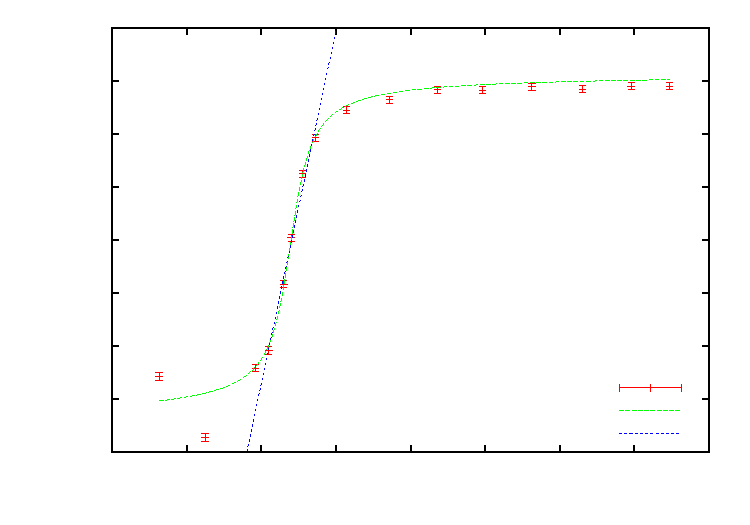
\includegraphics{phase}}%
    \gplfronttext
  \end{picture}%
\endgroup

	\caption{Phasenverschiebung des Serienresonanzkreises.}
	\label{fig:phase}
\end{figure}
Das Programm \textit{Gnuplot} liefert bei dem Theorie-Fit der Phasenverschiebung aus Formel \eqref{eq:phase_serie} für die drei Parameter $R$, $L$ und $C$ Fehler, die 30 mal so groß sind wie der eigentliche Wert.
Um dies zu beheben, setzt man den Wert für den Widerstand fest und fittet nur die anderen beiden Parameter (Abb.\ref{fig:phase}).
Dabei wird der Mittelwert $\overline R&=(80.3 \pm 0.5)\,\si{\ohm}$ aus den beiden obigen Werten verwendet.
Man erhält
\begin{align*}
	C &= (1.80 \pm 0.24)\,\si{\micro\farad}\qquad \text{und}\\
	L &= (390 \pm 50)\,\si{\milli\henry}\,.
\end{align*}
Die daraus mit \eqref{eq:omega_R} und \eqref{eq:omega_R_fehler} berechnete Resonanzfrequenz beträgt
\begin{empheq}[box=\shadowbox*]{align*}
	\omega_R&=(1200 \pm 110)\,\si\hertz \,.
\end{empheq}


Bei der Resonanzfrequenz verschwindet die Phasenverschiebung.
In diesem Bereich ist der Arcustangens in etwa linear.
So kann man zusätzlich zu dem Fit der Theoriekurve \eqref{eq:phase_serie} noch eine Gerade durch die Werte in der Nähe der Resonanzfrequenz legen.
Aus der Steigung $m=(6.7 \pm 0.5)\,\si{\per \hertz}$ und dem y-Achsenabschnitt $b=(-8.0 \pm 0.6)$ kann man mit
\begin{align}
	\omega_R&=\omega(\varphi=0)=- \frac{b}{m}\,,\\
	\sigma_{\omega_R}&=\frac{1}{m^{2}} \cdot \sqrt{b^{2} \cdot \sigma_{m}^{2} + m^{2} \cdot \sigma_{b}^{2}}
\end{align}
die Resonanzfrequenz berechnen.
Man erhält
\begin{empheq}[box=\shadowbox*]{align*}
	\omega_R&=(1200 \pm 120)\,\si\hertz \,.
\end{empheq}
\subsubsection{Teilspannungen}
\begin{figure}[!htb]
	\centering
	% GNUPLOT: LaTeX picture with Postscript
\begingroup
  \makeatletter
  \providecommand\color[2][]{%
    \GenericError{(gnuplot) \space\space\space\@spaces}{%
      Package color not loaded in conjunction with
      terminal option `colourtext'%
    }{See the gnuplot documentation for explanation.%
    }{Either use 'blacktext' in gnuplot or load the package
      color.sty in LaTeX.}%
    \renewcommand\color[2][]{}%
  }%
  \providecommand\includegraphics[2][]{%
    \GenericError{(gnuplot) \space\space\space\@spaces}{%
      Package graphicx or graphics not loaded%
    }{See the gnuplot documentation for explanation.%
    }{The gnuplot epslatex terminal needs graphicx.sty or graphics.sty.}%
    \renewcommand\includegraphics[2][]{}%
  }%
  \providecommand\rotatebox[2]{#2}%
  \@ifundefined{ifGPcolor}{%
    \newif\ifGPcolor
    \GPcolortrue
  }{}%
  \@ifundefined{ifGPblacktext}{%
    \newif\ifGPblacktext
    \GPblacktexttrue
  }{}%
  % define a \g@addto@macro without @ in the name:
  \let\gplgaddtomacro\g@addto@macro
  % define empty templates for all commands taking text:
  \gdef\gplbacktext{}%
  \gdef\gplfronttext{}%
  \makeatother
  \ifGPblacktext
    % no textcolor at all
    \def\colorrgb#1{}%
    \def\colorgray#1{}%
  \else
    % gray or color?
    \ifGPcolor
      \def\colorrgb#1{\color[rgb]{#1}}%
      \def\colorgray#1{\color[gray]{#1}}%
      \expandafter\def\csname LTw\endcsname{\color{white}}%
      \expandafter\def\csname LTb\endcsname{\color{black}}%
      \expandafter\def\csname LTa\endcsname{\color{black}}%
      \expandafter\def\csname LT0\endcsname{\color[rgb]{1,0,0}}%
      \expandafter\def\csname LT1\endcsname{\color[rgb]{0,1,0}}%
      \expandafter\def\csname LT2\endcsname{\color[rgb]{0,0,1}}%
      \expandafter\def\csname LT3\endcsname{\color[rgb]{1,0,1}}%
      \expandafter\def\csname LT4\endcsname{\color[rgb]{0,1,1}}%
      \expandafter\def\csname LT5\endcsname{\color[rgb]{1,1,0}}%
      \expandafter\def\csname LT6\endcsname{\color[rgb]{0,0,0}}%
      \expandafter\def\csname LT7\endcsname{\color[rgb]{1,0.3,0}}%
      \expandafter\def\csname LT8\endcsname{\color[rgb]{0.5,0.5,0.5}}%
    \else
      % gray
      \def\colorrgb#1{\color{black}}%
      \def\colorgray#1{\color[gray]{#1}}%
      \expandafter\def\csname LTw\endcsname{\color{white}}%
      \expandafter\def\csname LTb\endcsname{\color{black}}%
      \expandafter\def\csname LTa\endcsname{\color{black}}%
      \expandafter\def\csname LT0\endcsname{\color{black}}%
      \expandafter\def\csname LT1\endcsname{\color{black}}%
      \expandafter\def\csname LT2\endcsname{\color{black}}%
      \expandafter\def\csname LT3\endcsname{\color{black}}%
      \expandafter\def\csname LT4\endcsname{\color{black}}%
      \expandafter\def\csname LT5\endcsname{\color{black}}%
      \expandafter\def\csname LT6\endcsname{\color{black}}%
      \expandafter\def\csname LT7\endcsname{\color{black}}%
      \expandafter\def\csname LT8\endcsname{\color{black}}%
    \fi
  \fi
  \setlength{\unitlength}{0.0500bp}%
  \begin{picture}(7200.00,5040.00)%
    \gplgaddtomacro\gplbacktext{%
      \csname LTb\endcsname%
      \put(814,704){\makebox(0,0)[r]{\strut{} 0}}%
      \put(814,1383){\makebox(0,0)[r]{\strut{} 10}}%
      \put(814,2061){\makebox(0,0)[r]{\strut{} 20}}%
      \put(814,2740){\makebox(0,0)[r]{\strut{} 30}}%
      \put(814,3418){\makebox(0,0)[r]{\strut{} 40}}%
      \put(814,4097){\makebox(0,0)[r]{\strut{} 50}}%
      \put(814,4775){\makebox(0,0)[r]{\strut{} 60}}%
      \put(946,484){\makebox(0,0){\strut{} 0}}%
      \put(1678,484){\makebox(0,0){\strut{} 0.5}}%
      \put(2410,484){\makebox(0,0){\strut{} 1}}%
      \put(3142,484){\makebox(0,0){\strut{} 1.5}}%
      \put(3875,484){\makebox(0,0){\strut{} 2}}%
      \put(4607,484){\makebox(0,0){\strut{} 2.5}}%
      \put(5339,484){\makebox(0,0){\strut{} 3}}%
      \put(6071,484){\makebox(0,0){\strut{} 3.5}}%
      \put(6803,484){\makebox(0,0){\strut{} 4}}%
      \put(176,2739){\rotatebox{-270}{\makebox(0,0){\strut{}Spannung [V]}}}%
      \put(3874,154){\makebox(0,0){\strut{}$\omega$ [kHz]}}%
    }%
    \gplgaddtomacro\gplfronttext{%
      \csname LTb\endcsname%
      \put(5816,4602){\makebox(0,0)[r]{\strut{}$U$}}%
      \csname LTb\endcsname%
      \put(5816,4382){\makebox(0,0)[r]{\strut{}$U_{L+R}$}}%
      \csname LTb\endcsname%
      \put(5816,4162){\makebox(0,0)[r]{\strut{}$U_{C}$}}%
      \csname LTb\endcsname%
      \put(5816,3942){\makebox(0,0)[r]{\strut{}$U_C$-Fit}}%
    }%
    \gplbacktext
    \put(0,0){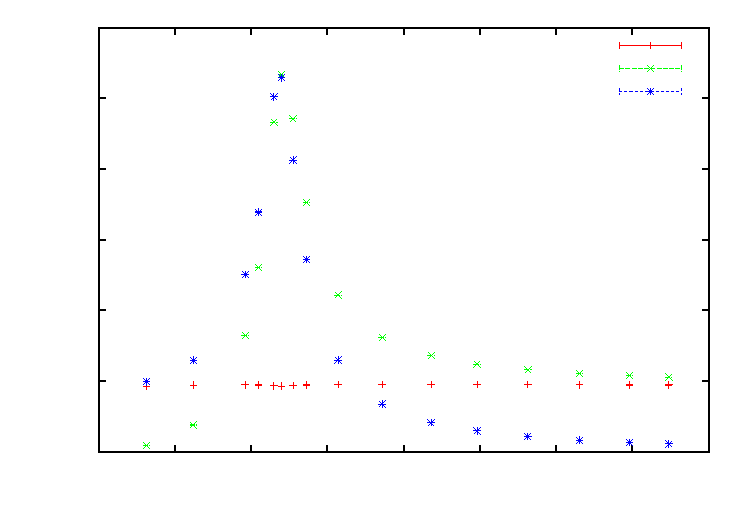
\includegraphics{spannungen}}%
    \gplfronttext
  \end{picture}%
\endgroup

	\caption{Teilspannungen und Gesamtspannung des Serienresonanzkreises in Abhängigkeit der Frequenz.}
	\label{fig:teilU}
\end{figure}
Trägt man die Teilspannungen $U_C$ und $U_{L+R}$ in Abhängigkeit der Frequenz auf (Abb. \ref{fig:teilU}), fällt auf, dass beide ihr Maximum bei der Resonanzfrequenz haben.
Außerdem ist dieses in etwa gleich groß.
Dies war zu erwarten, da sich dort kapazitiver Widerstand und induktiver Widerstand aufheben.
Dies kann man auch in der Abb. \ref{fig:zeigerU} erkennen.
Dort sind die Spannungen $U_C$ und $U_{L+R}$ sowie die Gesamtspannung $U$ maßstabsgetreu eingezeichnet, welche sich bei der Resonanzfrequenz ergeben.
Dazu werden die Messwerte bei einer gemessenen Phasenverschiebung von $1^\circ$ verwendet: $U=9.26\,$V, $U_C=52.9\,$V und $U_{L+R}=53.4\,$V. 
Der eingezeichnete Winkel $\varphi=\arccos\left(\frac{U}{U_{L+R}}\right)=80^\circ=1.396\,$rad ist die Phasenverschiebung zwischen $U_{L+R}$ und dem Strom $I$, da dieser bei $\omega_R$ mit $U$ in Phase ist.
Da hier kein kapazitiver Widerstand vorhanden ist, kann man diese Verschiebung auch mit der Formel \eqref{eq:phase_serie} ausrechnen. Dazu wird $C=0$ gesetzt:
\begin{align}
	\varphi=\arctan\left(\frac{\omega_R L}{R}\right)\,.
\end{align}
Da alle drei Größen fehlerbehaftet sind, folgt mit der Gauss'schen Fehlerfortpflanzung
\begin{align}	
	\sigma_{\varphi}=\frac{1}{(L \omega_R)^{2} + R^{2}} \cdot \sqrt{(LR)^{2}\, \sigma_{\omega_R}^{2} + (L \omega_R)^{2}\,\sigma_{R}^{2}  + (R \omega_R)^{2}\,\sigma_{L}^{2}}\,.
\end{align}
Für die gewichteten Mittelwerte $\overline{\omega_R}=(1199.9\pm 2.3)\,\si\hertz$, $\overline{R}=(80.3 \pm 0.5)\,\si\ohm$ und $\overline{L}=(386.2 \pm 0.6)\,\si{\milli\henry}$ aus den obigen Berechnungen ergibt sich eine Phasenverschiebung von
\begin{align*}
	\varphi=(1.399 \pm 0.001)\,\si{rad}\,.
\end{align*}
Es ergibt sich eine Abweichung von $2\permil$.
\begin{figure}
	\centering	
	\adjustbox{height=0.4\textheight}{\input{SpannungenZeiger.pdf_tex}}
	\caption{Zeigerdiagramm der Spannungen $U$, $U_C$ und $U_{L+R}$ der Serienschaltung bei der Resonanzfrequenz}
	\label{fig:zeigerU}
\end{figure}

\subsection{Parallelkreis}
\begin{figure}[!htb]
	\centering
	% GNUPLOT: LaTeX picture with Postscript
\begingroup
  \makeatletter
  \providecommand\color[2][]{%
    \GenericError{(gnuplot) \space\space\space\@spaces}{%
      Package color not loaded in conjunction with
      terminal option `colourtext'%
    }{See the gnuplot documentation for explanation.%
    }{Either use 'blacktext' in gnuplot or load the package
      color.sty in LaTeX.}%
    \renewcommand\color[2][]{}%
  }%
  \providecommand\includegraphics[2][]{%
    \GenericError{(gnuplot) \space\space\space\@spaces}{%
      Package graphicx or graphics not loaded%
    }{See the gnuplot documentation for explanation.%
    }{The gnuplot epslatex terminal needs graphicx.sty or graphics.sty.}%
    \renewcommand\includegraphics[2][]{}%
  }%
  \providecommand\rotatebox[2]{#2}%
  \@ifundefined{ifGPcolor}{%
    \newif\ifGPcolor
    \GPcolortrue
  }{}%
  \@ifundefined{ifGPblacktext}{%
    \newif\ifGPblacktext
    \GPblacktexttrue
  }{}%
  % define a \g@addto@macro without @ in the name:
  \let\gplgaddtomacro\g@addto@macro
  % define empty templates for all commands taking text:
  \gdef\gplbacktext{}%
  \gdef\gplfronttext{}%
  \makeatother
  \ifGPblacktext
    % no textcolor at all
    \def\colorrgb#1{}%
    \def\colorgray#1{}%
  \else
    % gray or color?
    \ifGPcolor
      \def\colorrgb#1{\color[rgb]{#1}}%
      \def\colorgray#1{\color[gray]{#1}}%
      \expandafter\def\csname LTw\endcsname{\color{white}}%
      \expandafter\def\csname LTb\endcsname{\color{black}}%
      \expandafter\def\csname LTa\endcsname{\color{black}}%
      \expandafter\def\csname LT0\endcsname{\color[rgb]{1,0,0}}%
      \expandafter\def\csname LT1\endcsname{\color[rgb]{0,1,0}}%
      \expandafter\def\csname LT2\endcsname{\color[rgb]{0,0,1}}%
      \expandafter\def\csname LT3\endcsname{\color[rgb]{1,0,1}}%
      \expandafter\def\csname LT4\endcsname{\color[rgb]{0,1,1}}%
      \expandafter\def\csname LT5\endcsname{\color[rgb]{1,1,0}}%
      \expandafter\def\csname LT6\endcsname{\color[rgb]{0,0,0}}%
      \expandafter\def\csname LT7\endcsname{\color[rgb]{1,0.3,0}}%
      \expandafter\def\csname LT8\endcsname{\color[rgb]{0.5,0.5,0.5}}%
    \else
      % gray
      \def\colorrgb#1{\color{black}}%
      \def\colorgray#1{\color[gray]{#1}}%
      \expandafter\def\csname LTw\endcsname{\color{white}}%
      \expandafter\def\csname LTb\endcsname{\color{black}}%
      \expandafter\def\csname LTa\endcsname{\color{black}}%
      \expandafter\def\csname LT0\endcsname{\color{black}}%
      \expandafter\def\csname LT1\endcsname{\color{black}}%
      \expandafter\def\csname LT2\endcsname{\color{black}}%
      \expandafter\def\csname LT3\endcsname{\color{black}}%
      \expandafter\def\csname LT4\endcsname{\color{black}}%
      \expandafter\def\csname LT5\endcsname{\color{black}}%
      \expandafter\def\csname LT6\endcsname{\color{black}}%
      \expandafter\def\csname LT7\endcsname{\color{black}}%
      \expandafter\def\csname LT8\endcsname{\color{black}}%
    \fi
  \fi
  \setlength{\unitlength}{0.0500bp}%
  \begin{picture}(7200.00,5040.00)%
    \gplgaddtomacro\gplbacktext{%
      \csname LTb\endcsname%
      \put(1254,704){\makebox(0,0)[r]{\strut{}-0.5}}%
      \put(1254,1156){\makebox(0,0)[r]{\strut{} 0}}%
      \put(1254,1609){\makebox(0,0)[r]{\strut{} 0.5}}%
      \put(1254,2061){\makebox(0,0)[r]{\strut{} 1}}%
      \put(1254,2514){\makebox(0,0)[r]{\strut{} 1.5}}%
      \put(1254,2966){\makebox(0,0)[r]{\strut{} 2}}%
      \put(1254,3419){\makebox(0,0)[r]{\strut{} 2.5}}%
      \put(1254,3871){\makebox(0,0)[r]{\strut{} 3}}%
      \put(1254,4324){\makebox(0,0)[r]{\strut{} 3.5}}%
      \put(1254,4776){\makebox(0,0)[r]{\strut{} 4}}%
      \put(1386,484){\makebox(0,0){\strut{} 0}}%
      \put(2083,484){\makebox(0,0){\strut{} 500}}%
      \put(2779,484){\makebox(0,0){\strut{} 1000}}%
      \put(3476,484){\makebox(0,0){\strut{} 1500}}%
      \put(4172,484){\makebox(0,0){\strut{} 2000}}%
      \put(4869,484){\makebox(0,0){\strut{} 2500}}%
      \put(5565,484){\makebox(0,0){\strut{} 3000}}%
      \put(6262,484){\makebox(0,0){\strut{} 3500}}%
      \put(6958,484){\makebox(0,0){\strut{} 4000}}%
      \put(484,2740){\rotatebox{90}{\makebox(0,0){\strut{}Impedanz [$\Omega$]}}}%
      \put(4172,154){\makebox(0,0){\strut{}Kreisfrequenz [Hz]}}%
    }%
    \gplgaddtomacro\gplfronttext{%
      \csname LTb\endcsname%
      \put(5971,4603){\makebox(0,0)[r]{\strut{}Messwerte}}%
    }%
    \gplbacktext
    \put(0,0){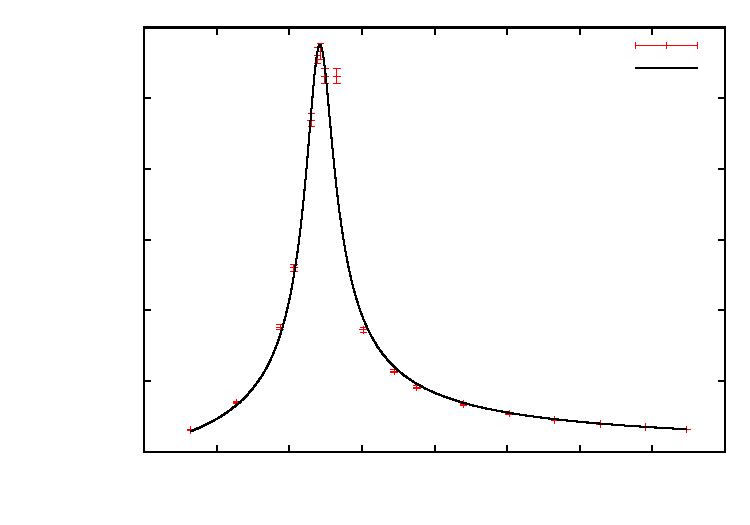
\includegraphics{messung3}}%
    \gplfronttext
  \end{picture}%
\endgroup

	\caption{Scheinwiderstand des Parallelkreises als Funktion der Kreisfrequenz.}
	\label{fig:messung3}
\end{figure}
In Abb. \ref{fig:messung3} ist der Scheinwiderstand des Parallelkreises gegen die Frequenz aufgetragen.
Der Fit der Theoriekurve \eqref{eq:parallel} liefert 
\begin{align*}
	R_L &= (68\pm 5)\,\si{\ohm}\,,\\
	L &= (370 \pm 10)\,\si{\milli\henry}\qquad \text{und}\\
	C &= (1.88  \pm 0.05)\, \si{\micro\farad}\,.
\end{align*}
Daraus ergibt sich mit \eqref{eq:omega_R} und \eqref{eq:omega_R_fehler} die Resonanzfrequenz des Serienschwingkreises
\begin{empheq}[box=\shadowbox*]{align*}
	\omega_R&=(1199 \pm 23)\,\si\hertz \,.
\end{empheq}


\section{Diskussion}
\label{sec:diskussion}
\subsection{Ohmscher Widerstand}
Mit dem Multimeter wurde für den einzelne ohmsche Widerstand der Wert $R_\Omega=(10.1 \pm 0.1)\,\Omega$, für den Widerstand der Spule der Wert $R_L=(65.1 \pm 0.1)\,\Omega$ gemessen.
Als Summe ergibt sich $R=(75.2 \pm 0.2)\,\Omega$.
Verglichen mit dem Mittelwert $R=(80.3 \pm 0.5)\,\si\ohm$ aus den obigen Messungen ergibt sich eine Differenz von etwa $5\,\Omega$.
Diese ist mit dem Innenwiderstand des Amperemeters erklärbar.
Aus der Parallelkreis-Messung ergibt sich der Widerstand der Spule $R_L=(68\pm 5)\,\si{\ohm}$.
Dieser Wert weist eine Abweichung von $5\%$ zu dem vom Multimeter gemessenen Wert auf.
Jedoch liegt letzterer Wert im Fehlerintervall des durch den Fit bestimmten Widerstandes.

\subsection{Induktivität}
Die Bestimmung der Induktivität weist eine große Konsistenz auf:
Der Mittelwert $L=(386.2 \pm 0.6)\,\si{\milli\henry}$ liegt in fast allen Fehlerintervallen. Lediglich der über die Parallelschaltung bestimmte Wert ist etwa $5\%$ zu klein.
Die Werte aus den Fits von Abb. \ref{fig:messung1} und \ref{fig:messung2} sind am genausten.
Die Spule hat eine Windungszahl $n=1000$ und einen Durchmesser $\diameter=233\,$mm.
Zwar wurde die Länge nicht gemessen, sie ist jedoch kleiner als der Durchmesser.
So kann die Induktivität nicht mit der Formel für lange Spulen berechnet werden, da Randeffekte betrachtet werden müssen.
Es wäre interessant gewesen, die bestimmte Induktivität mit einem aus den Spulendaten berechneten Wert zu vergleichen.
 
\subsection{Kapazität}
Für die Kapazität ergibt sich aus allen obigen Messungen  der gewichtete Mittelwert $C=(1.800 \pm 0.005)\,\si{\micro\farad}$.
Mit dem Multimeter wurde der Wert $C=(1.806 \pm 0.010)\,\si{\micro\farad}$ gemessen.
Dieser ist zwar etwa $4\permil$ größer, jedoch liegt der berechnete Wert im Fehlerintervall und der Multimeter-Wert liegt nur knapp außerhalb des berechneten Fehlerintervalls.
Betrachtet man die durch die einzelnen Bestimmungsmethoden berechneten Werte genauer, erkennt man, dass der Wert aus dem Parallelkreis-Fit die größte Abweichung von etwa $5\%$ besitzt, der Wert aus der Phasenverschiebung die größte Ungenauigkeit aufweist.

\subsection{Resonanzfrequenz}
Bei der Bestimmung der Resonanzfrequenz ist auffällig, dass alle Werte bei ziemlich genau $1200\,$Hz liegen.
Nur die Fehler haben verschiedene Größenordnungen:
So ist der Wert aus dem Scheinwiderstands-Fit der Serienschaltung (Abb. \ref{fig:messung2}) mit einem Fehler von $2.3\,$Hz am genausten, die beiden Werte aus der Phasenverschiebung weisen einen sehr großen Fehler von über $100\,$Hz auf.
Es wäre möglich, dass dies an der jeweils gefitteten Funktion liegt.
So ist es auch nicht verwunderlich, dass der Fit nach der Formel \eqref{eq:phase_serie} -- wie oben schon erwähnt -- sehr große Fehler liefert:
Die Resonanzfrequenz hängt nämlich nur von dem Produkt $LC$ ab.
Wenn die Induktivität größer wäre, die Kapazität um den gleichen Faktor jedoch kleiner,  so ändert dies nichts an der Resonanzfrequenz.
Der Widerstand $R$ bestimmt dann, wie schnell sich die Phasenverschiebung an die Extrema $\varphi=\pm\frac{\pi}{2}$ annähert.

\bibliography{literatur}
\bibliographystyle{babalpha}
\end{document}
